% Options for packages loaded elsewhere
\PassOptionsToPackage{unicode}{hyperref}
\PassOptionsToPackage{hyphens}{url}
%
\documentclass[
  5pt,
  ignorenonframetext,
]{beamer}
\usepackage{pgfpages}
\setbeamertemplate{caption}[numbered]
\setbeamertemplate{caption label separator}{: }
\setbeamercolor{caption name}{fg=normal text.fg}
\beamertemplatenavigationsymbolsempty
% Prevent slide breaks in the middle of a paragraph
\widowpenalties 1 10000
\raggedbottom
\setbeamertemplate{part page}{
  \centering
  \begin{beamercolorbox}[sep=16pt,center]{part title}
    \usebeamerfont{part title}\insertpart\par
  \end{beamercolorbox}
}
\setbeamertemplate{section page}{
  \centering
  \begin{beamercolorbox}[sep=12pt,center]{part title}
    \usebeamerfont{section title}\insertsection\par
  \end{beamercolorbox}
}
\setbeamertemplate{subsection page}{
  \centering
  \begin{beamercolorbox}[sep=8pt,center]{part title}
    \usebeamerfont{subsection title}\insertsubsection\par
  \end{beamercolorbox}
}
\AtBeginPart{
  \frame{\partpage}
}
\AtBeginSection{
  \ifbibliography
  \else
    \frame{\sectionpage}
  \fi
}
\AtBeginSubsection{
  \frame{\subsectionpage}
}
\usepackage{lmodern}
\usepackage{amssymb,amsmath}
\usepackage{ifxetex,ifluatex}
\ifnum 0\ifxetex 1\fi\ifluatex 1\fi=0 % if pdftex
  \usepackage[T1]{fontenc}
  \usepackage[utf8]{inputenc}
  \usepackage{textcomp} % provide euro and other symbols
\else % if luatex or xetex
  \usepackage{unicode-math}
  \defaultfontfeatures{Scale=MatchLowercase}
  \defaultfontfeatures[\rmfamily]{Ligatures=TeX,Scale=1}
\fi
\usetheme[]{Berlin}
\usecolortheme{beaver}
\usefonttheme{structurebold}
% Use upquote if available, for straight quotes in verbatim environments
\IfFileExists{upquote.sty}{\usepackage{upquote}}{}
\IfFileExists{microtype.sty}{% use microtype if available
  \usepackage[]{microtype}
  \UseMicrotypeSet[protrusion]{basicmath} % disable protrusion for tt fonts
}{}
\makeatletter
\@ifundefined{KOMAClassName}{% if non-KOMA class
  \IfFileExists{parskip.sty}{%
    \usepackage{parskip}
  }{% else
    \setlength{\parindent}{0pt}
    \setlength{\parskip}{6pt plus 2pt minus 1pt}}
}{% if KOMA class
  \KOMAoptions{parskip=half}}
\makeatother
\usepackage{xcolor}
\IfFileExists{xurl.sty}{\usepackage{xurl}}{} % add URL line breaks if available
\IfFileExists{bookmark.sty}{\usepackage{bookmark}}{\usepackage{hyperref}}
\hypersetup{
  pdftitle={Seminar},
  hidelinks,
  pdfcreator={LaTeX via pandoc}}
\urlstyle{same} % disable monospaced font for URLs
\newif\ifbibliography
\usepackage{longtable,booktabs}
\usepackage{caption}
% Make caption package work with longtable
\makeatletter
\def\fnum@table{\tablename~\thetable}
\makeatother
\setlength{\emergencystretch}{3em} % prevent overfull lines
\providecommand{\tightlist}{%
  \setlength{\itemsep}{0pt}\setlength{\parskip}{0pt}}
\setcounter{secnumdepth}{-\maxdimen} % remove section numbering
\usepackage[orientation = landscape, size = custom, width = 16, height = 9, scale = 0.5]{beamerposter}
\setbeamertemplate{footline}[frame number]
\usefonttheme{serif}
% ## ---------------------------------------------------------------------- 
% \setbeamerfont{supervisor}{size = \scriptsize}
% \setbeamerfont{instructor}{size = \scriptsize}
% ## ---------------------------------------------------------------------- 
\defbeamertemplate{title page}{RunTemplate}
{
  \vfill
  % ## ---------------------------------------------------------------------- 
  \begin{beamercolorbox}[sep = 10pt, center]{titleGraph}
    \inserttitlegraphic
  \end{beamercolorbox}
  % ## ---------------------------------------------------------------------- 
  \begin{beamercolorbox}[sep = 8pt, center, rounded = true]{title}
    \usebeamerfont{title}\inserttitle\par
    \ifx\insertsubtitle\@empty
  \else
  {\usebeamerfont{subtitle}\usebeamercolor[fg]{subtitle}\insertsubtitle\par}
  \fi
  \end{beamercolorbox}
  % ## ---------------------------------------------------------------------- 
  \vskip0.4em
  % ## ---------------------------------------------------------------------- 
  \begin{beamercolorbox}[sep = 8pt, center]{author}
    \usebeamerfont{author}\insertauthor\par
  \end{beamercolorbox}
  % ## ---------------------------------------------------------------------- 
  % \begin{beamercolorbox}[sep = 5pt, center]{supervisor}
    % \usebeamerfont{supervisor}Supervisor: \supervisor
  % \end{beamercolorbox}
  % ## ---------------------------------------------------------------------- 
  % \begin{beamercolorbox}[sep = 5pt, center]{instructor}
    % \usebeamerfont{instructor}\instructor
  % \end{beamercolorbox}
  % ## ---------------------------------------------------------------------- 
  \begin{beamercolorbox}[sep = 8pt, center]{institute}
    \usebeamerfont{institute}\insertinstitute\par
  \end{beamercolorbox}
  % ## ---------------------------------------------------------------------- 
  \begin{beamercolorbox}[sep = 8pt, center]{date}
    \usebeamerfont{date}\insertdate\par
  \end{beamercolorbox}
  \vfill
}
\setbeamertemplate{title page}[RunTemplate]

\newenvironment{cols}[1][]{}{}

\newenvironment{col}[1]{\begin{minipage}{#1}\ignorespaces}{%
\end{minipage}
\ifhmode\unskip\fi
\aftergroup\useignorespacesandallpars}

\def\useignorespacesandallpars#1\ignorespaces\fi{%
#1\fi\ignorespacesandallpars}

\makeatletter
\def\ignorespacesandallpars{%
  \@ifnextchar\par
    {\expandafter\ignorespacesandallpars\@gobble}%
    {}%
}
\makeatother
\AtBeginEnvironment{longtable}{\tiny} \titlegraphic{\centering 
\includegraphics{./logo_lixiao.png}} \usepackage{caption} \captionsetup{font={tiny}} \usepackage{setspace} \setstretch{1.3} \linespread{1.3}

\title{Seminar}
\author{Lichuang Huang}
\date{2023-07-12}
\institute{Wie-Biotech}

\begin{document}
\frame{\titlepage}

\hypertarget{repetition-of-technology}{%
\section{Repetition of Technology}\label{repetition-of-technology}}

\begin{frame}{Article}
\protect\hypertarget{article}{}
\includegraphics[width=135mm]{~/Pictures/Screenshots/Screenshot from 2023-07-11 10-24-38.png}

\tiny

Yang Q, et al.~(2017). \emph{Journal of Cachexia, Sarcopenia and
Muscle}.\vspace{0.5em} \newline
\end{frame}

\begin{frame}{Research idea}
\protect\hypertarget{research-idea}{}
\begin{cols}

\begin{col}{0.3\textwidth}

\begin{itemize}
\tightlist
\item
  Main

  \begin{itemize}
  \tightlist
  \item
    Identification
  \item
    Quantification
  \item
    Feature selection
  \item
    Establish model
  \item
    Validation
  \end{itemize}
\end{itemize}

\end{col}

\begin{col}{0.6\textwidth}
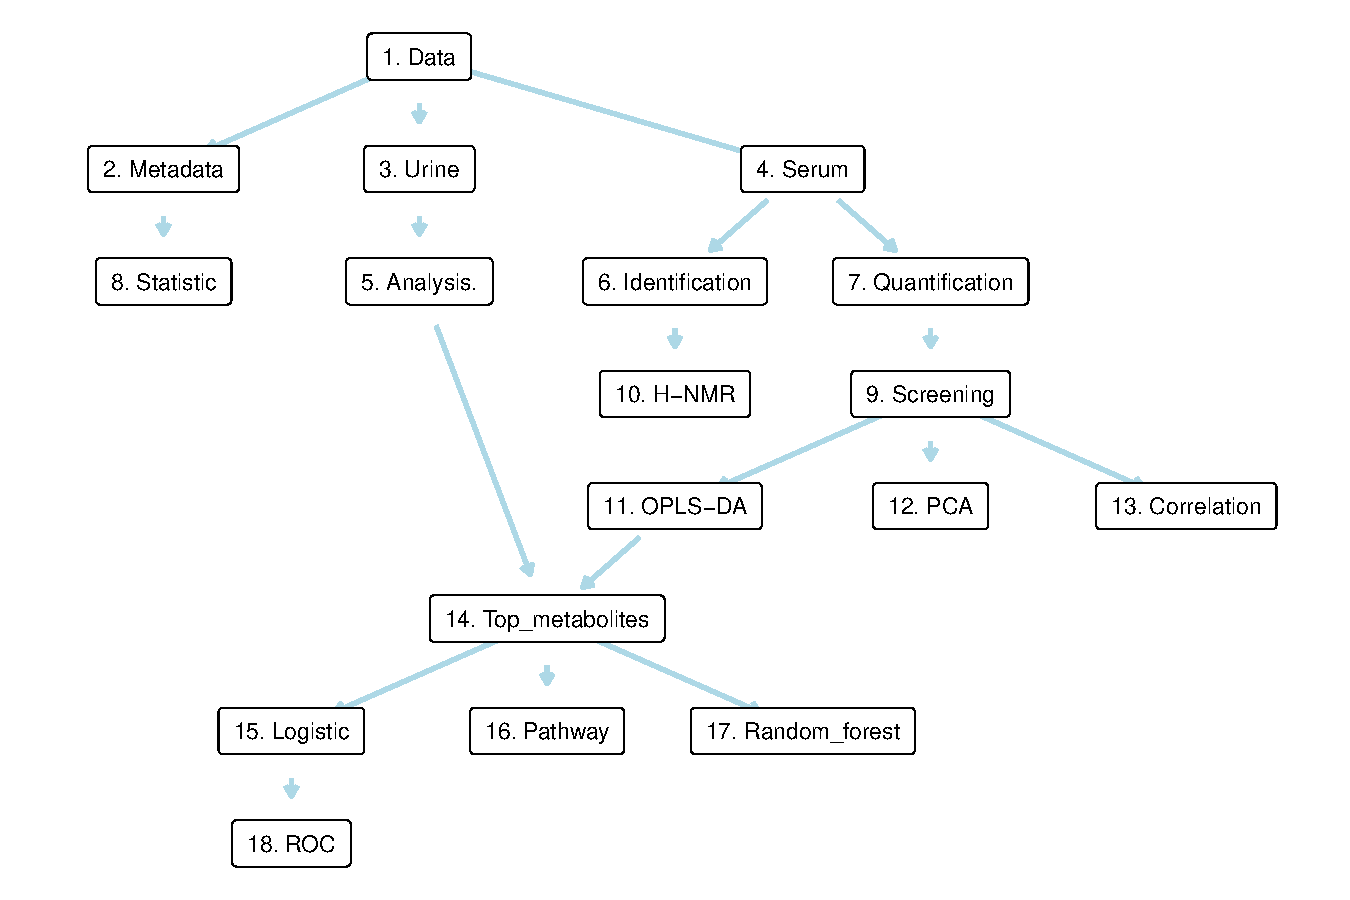
\includegraphics[height=65mm]{./figs/idea.pdf}

\end{col}

\end{cols}
\end{frame}

\begin{frame}[fragile]{Statistic of metadata}
\protect\hypertarget{statistic-of-metadata}{}
\begin{cols}

\begin{col}{0.4\textwidth}

\begin{itemize}
\tightlist
\item
  The pre-test

  \begin{enumerate}
  \tightlist
  \item
    Normal distribution

    \begin{itemize}
    \tightlist
    \item
      \texttt{shapiro.test()}
    \end{itemize}
  \item
    Variance test

    \begin{itemize}
    \tightlist
    \item
      \texttt{bartlett.test()}
    \end{itemize}
  \end{enumerate}
\item
  ANOVA

  \begin{itemize}
  \tightlist
  \item
    \texttt{aov()}
  \end{itemize}
\item
  Multiple comparison

  \begin{itemize}
  \tightlist
  \item
    \texttt{TurkeyHSD()}
  \end{itemize}
\end{itemize}

\end{col}

\begin{col}{0.6\textwidth}
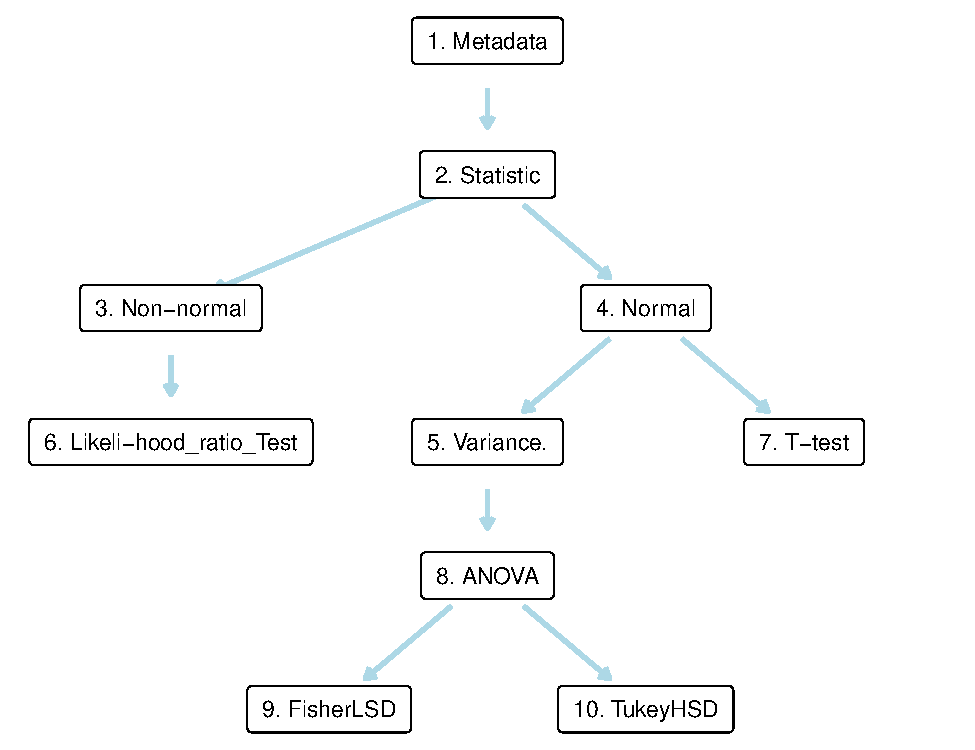
\includegraphics[height=65mm]{./figs/idea_ex.pdf}

\end{col}

\end{cols}
\end{frame}

\begin{frame}{Demo statistic}
\protect\hypertarget{demo-statistic}{}
\begin{cols}

\begin{col}{0.5\textwidth}

\begin{longtable}[]{@{}llr@{}}
\caption{Demo data}\tabularnewline
\toprule
sample & group & Total.cholesterol\tabularnewline
\midrule
\endfirsthead
\toprule
sample & group & Total.cholesterol\tabularnewline
\midrule
\endhead
Ca1 & Cachexia & 4.24\tabularnewline
Ca2 & Cachexia & 6.00\tabularnewline
Ca3 & Cachexia & NA\tabularnewline
Ca4 & Cachexia & NA\tabularnewline
Ca5 & Cachexia & 4.96\tabularnewline
T1 & cancer & 3.88\tabularnewline
T2 & cancer & 1.79\tabularnewline
T3 & cancer & 3.36\tabularnewline
T4 & cancer & 2.97\tabularnewline
T5 & cancer & 5.41\tabularnewline
Pro1 & Procachexia & 3.30\tabularnewline
Pro2 & Procachexia & 5.44\tabularnewline
Pro3 & Procachexia & NA\tabularnewline
\bottomrule
\end{longtable}

\end{col}

\begin{col}{0.5\textwidth}
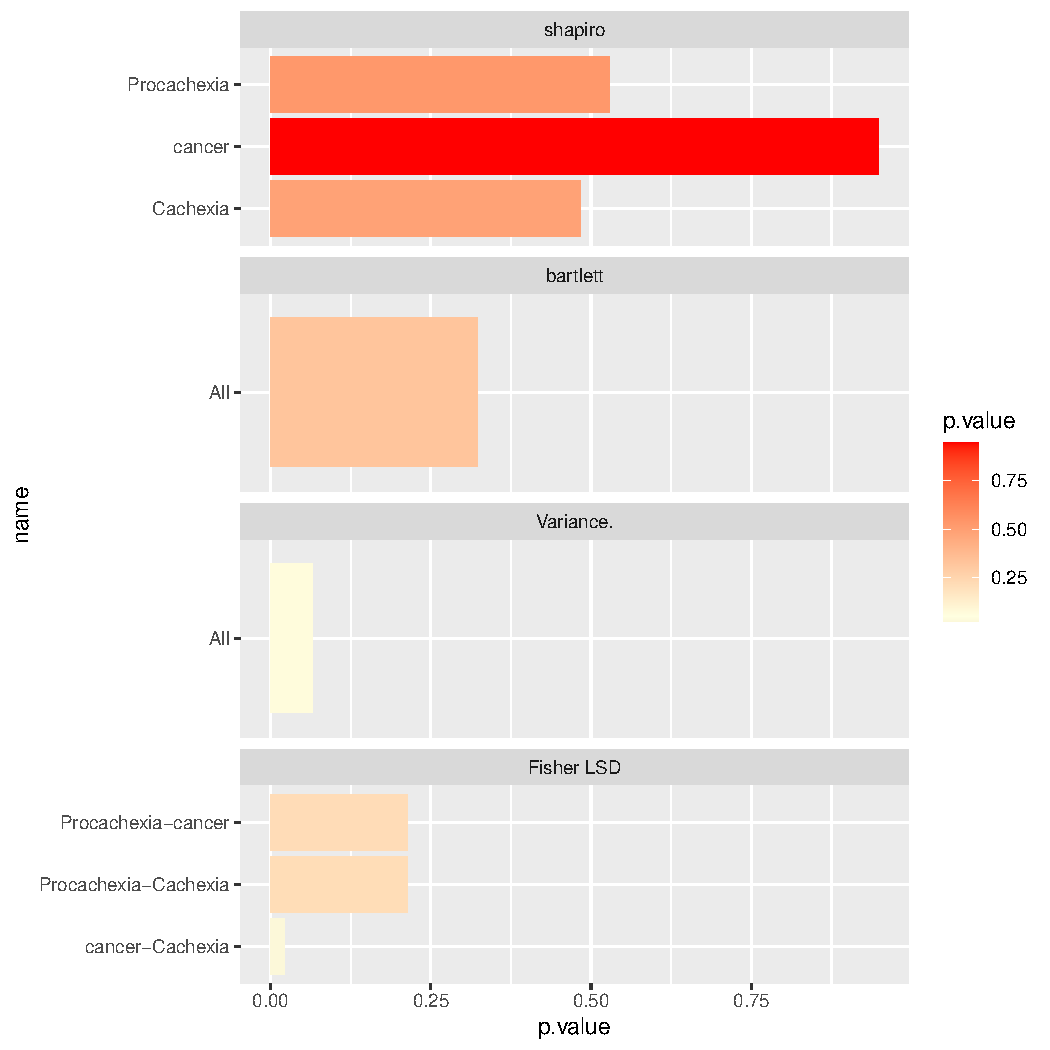
\includegraphics[height=62mm]{./figs/var_p.pdf}

\end{col}

\end{cols}
\end{frame}

\begin{frame}{Multivariate statistics: PCA}
\protect\hypertarget{multivariate-statistics-pca}{}
\begin{cols}

\begin{col}{0.6\textwidth}

\begin{longtable}[]{@{}rrrrl@{}}
\caption{Demo data}\tabularnewline
\toprule
Sepal.Length & Sepal.Width & Petal.Length & Petal.Width &
Species\tabularnewline
\midrule
\endfirsthead
\toprule
Sepal.Length & Sepal.Width & Petal.Length & Petal.Width &
Species\tabularnewline
\midrule
\endhead
5.1 & 3.5 & 1.4 & 0.2 & setosa\tabularnewline
4.9 & 3.0 & 1.4 & 0.2 & setosa\tabularnewline
4.7 & 3.2 & 1.3 & 0.2 & setosa\tabularnewline
4.6 & 3.1 & 1.5 & 0.2 & setosa\tabularnewline
7.0 & 3.2 & 4.7 & 1.4 & versicolor\tabularnewline
6.4 & 3.2 & 4.5 & 1.5 & versicolor\tabularnewline
6.9 & 3.1 & 4.9 & 1.5 & versicolor\tabularnewline
5.5 & 2.3 & 4.0 & 1.3 & versicolor\tabularnewline
6.3 & 3.3 & 6.0 & 2.5 & virginica\tabularnewline
5.8 & 2.7 & 5.1 & 1.9 & virginica\tabularnewline
7.1 & 3.0 & 5.9 & 2.1 & virginica\tabularnewline
6.3 & 2.9 & 5.6 & 1.8 & virginica\tabularnewline
\bottomrule
\end{longtable}

\end{col}

\begin{col}{0.02\textwidth}

\hspace{1pt}

\end{col}

\begin{col}{0.5\textwidth}
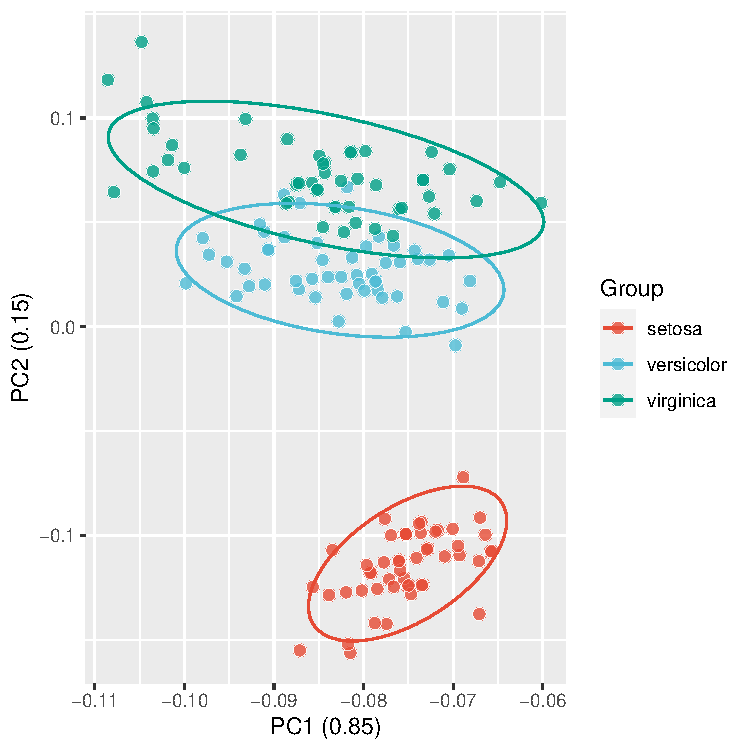
\includegraphics[height=60mm]{./figs/pca.pdf}

\end{col}

\end{cols}
\end{frame}

\begin{frame}{Multivariate statistics: OPLS-DA}
\protect\hypertarget{multivariate-statistics-opls-da}{}
\begin{cols}

\begin{col}{0.5\textwidth}
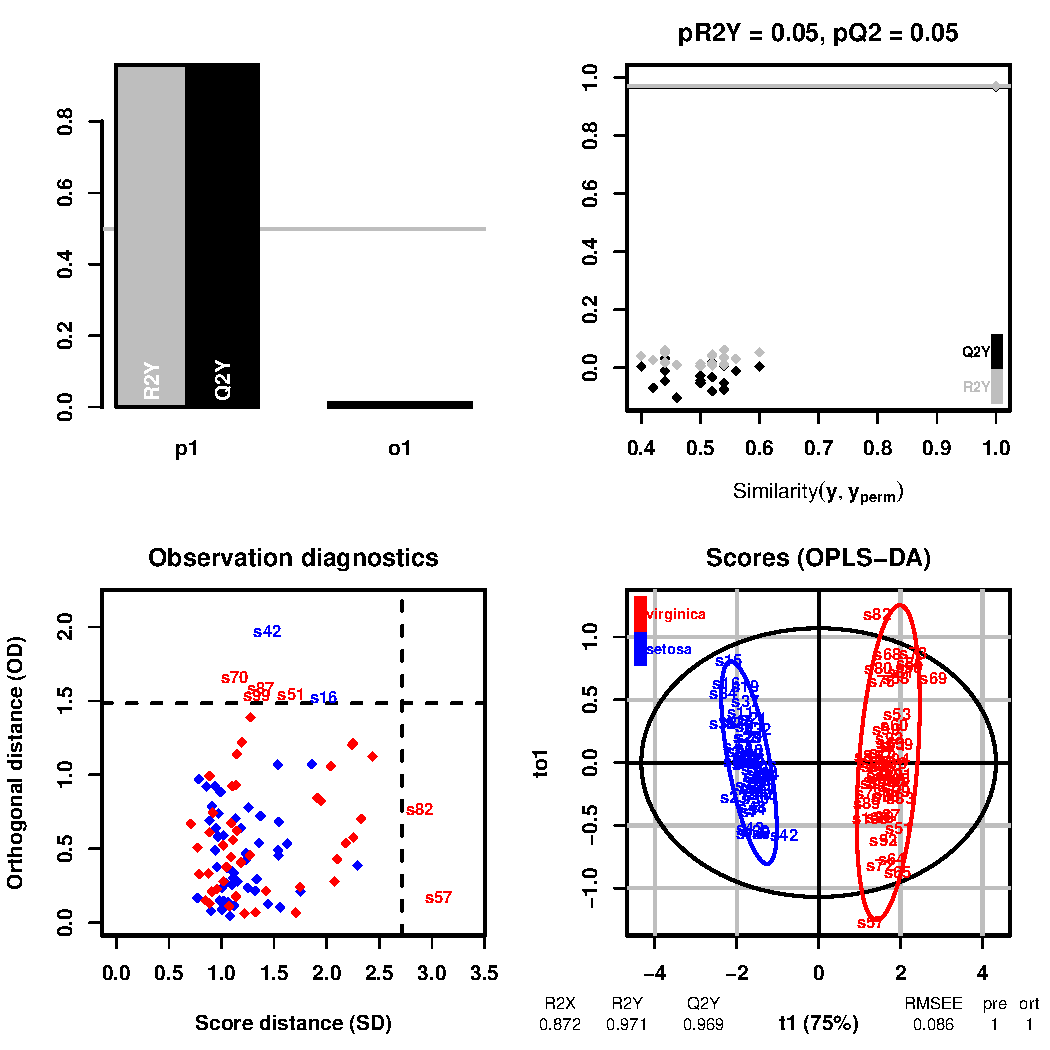
\includegraphics[height=65mm]{./figs/opls_form.pdf}

\end{col}

\begin{col}{0.5\textwidth}
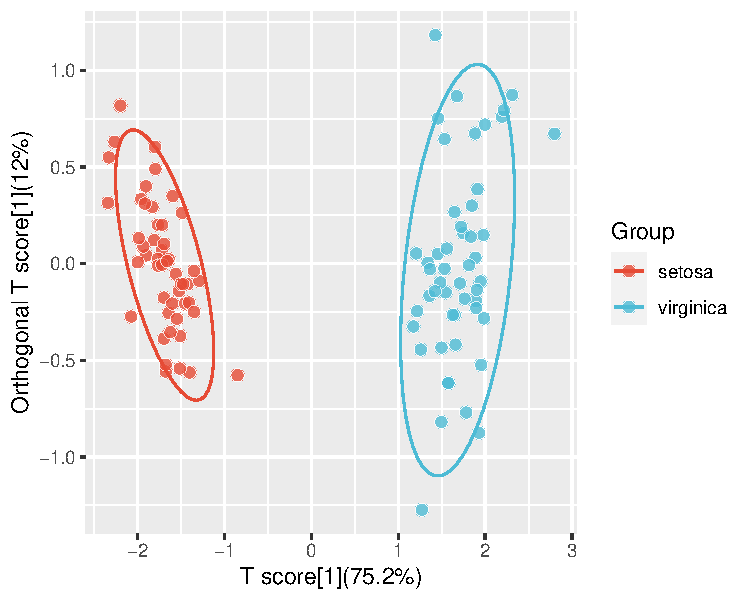
\includegraphics[height=65mm]{./figs/opls.pdf}

\end{col}

\end{cols}
\end{frame}

\begin{frame}{Random Forest}
\protect\hypertarget{random-forest}{}
\begin{cols}

\begin{col}{0.6\textwidth}

\begin{longtable}[]{@{}rrrrl@{}}
\caption{Traning data}\tabularnewline
\toprule
Sepal.Length & Sepal.Width & Petal.Length & Petal.Width &
Species\tabularnewline
\midrule
\endfirsthead
\toprule
Sepal.Length & Sepal.Width & Petal.Length & Petal.Width &
Species\tabularnewline
\midrule
\endhead
5.1 & 3.5 & 1.4 & 0.2 & setosa\tabularnewline
4.9 & 3.0 & 1.4 & 0.2 & setosa\tabularnewline
4.7 & 3.2 & 1.3 & 0.2 & setosa\tabularnewline
4.6 & 3.1 & 1.5 & 0.2 & setosa\tabularnewline
7.0 & 3.2 & 4.7 & 1.4 & versicolor\tabularnewline
6.4 & 3.2 & 4.5 & 1.5 & versicolor\tabularnewline
6.9 & 3.1 & 4.9 & 1.5 & versicolor\tabularnewline
5.5 & 2.3 & 4.0 & 1.3 & versicolor\tabularnewline
6.3 & 3.3 & 6.0 & 2.5 & virginica\tabularnewline
5.8 & 2.7 & 5.1 & 1.9 & virginica\tabularnewline
7.1 & 3.0 & 5.9 & 2.1 & virginica\tabularnewline
6.3 & 2.9 & 5.6 & 1.8 & virginica\tabularnewline
\bottomrule
\end{longtable}

\end{col}

\begin{col}{0.4\textwidth}
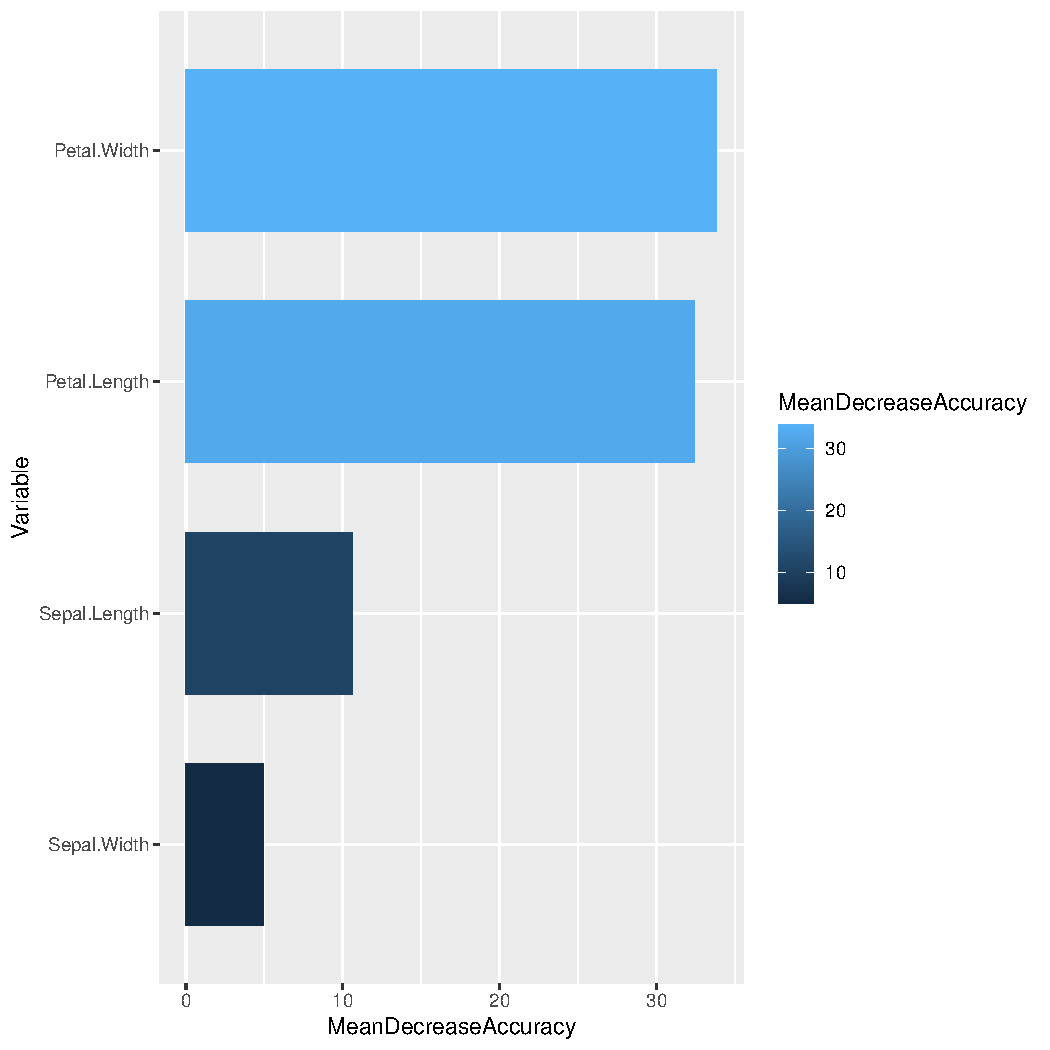
\includegraphics[height=65mm]{./figs/rf.pdf}

\end{col}

\end{cols}
\end{frame}

\begin{frame}{Logistic regression}
\protect\hypertarget{logistic-regression}{}
\begin{cols}

\begin{col}{0.5\textwidth}

\begin{longtable}[]{@{}rrrrl@{}}
\caption{Traning data}\tabularnewline
\toprule
Sepal.Length & Sepal.Width & Petal.Length & Petal.Width &
Species\tabularnewline
\midrule
\endfirsthead
\toprule
Sepal.Length & Sepal.Width & Petal.Length & Petal.Width &
Species\tabularnewline
\midrule
\endhead
5.1 & 3.5 & 1.4 & 0.2 & setosa\tabularnewline
4.9 & 3.0 & 1.4 & 0.2 & setosa\tabularnewline
4.7 & 3.2 & 1.3 & 0.2 & setosa\tabularnewline
4.6 & 3.1 & 1.5 & 0.2 & setosa\tabularnewline
\bottomrule
\end{longtable}

\begin{longtable}[]{@{}rrrr@{}}
\caption{Validate data}\tabularnewline
\toprule
Sepal.Length & Sepal.Width & Petal.Length & Petal.Width\tabularnewline
\midrule
\endfirsthead
\toprule
Sepal.Length & Sepal.Width & Petal.Length & Petal.Width\tabularnewline
\midrule
\endhead
5.85 & 2.94 & 4.32 & 1.34\tabularnewline
5.74 & 2.98 & 3.98 & 1.02\tabularnewline
5.04 & 3.41 & 3.52 & 0.90\tabularnewline
5.49 & 2.79 & 4.06 & 1.11\tabularnewline
\bottomrule
\end{longtable}

\end{col}

\begin{col}{0.4\textwidth}
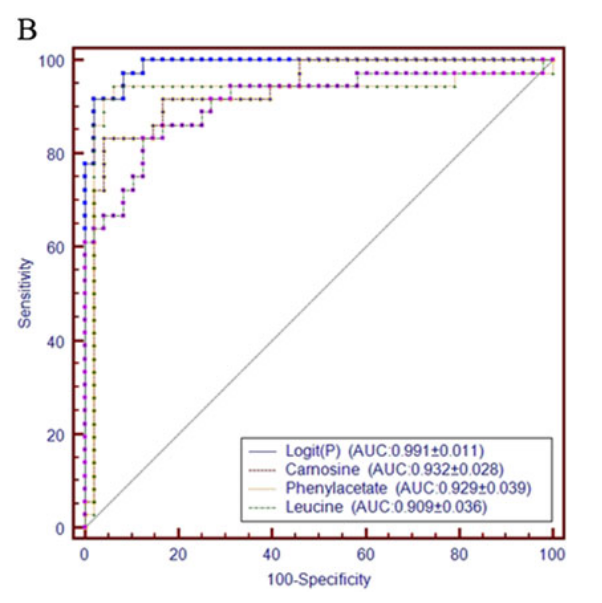
\includegraphics[height=65mm]{./figs/roc.png}

\end{col}

\end{cols}
\end{frame}

\hypertarget{thank-you}{%
\section{Thank you}\label{thank-you}}

\end{document}
